Dans cette section, nous présentons la conception détaillée des fonctionnalités développées au cours du sprint, à travers des diagrammes de classes et de séquences.
\subsubsection{Diagramme de classe du Sprint 2.1}
    Ce diagramme vient enrichir l'architecture définie au sprint précédent, en intégrant la gestion des tests fonctionnels automatisés et les analyses SEO avancées.
    \begin{figure}[H]
        \centering
        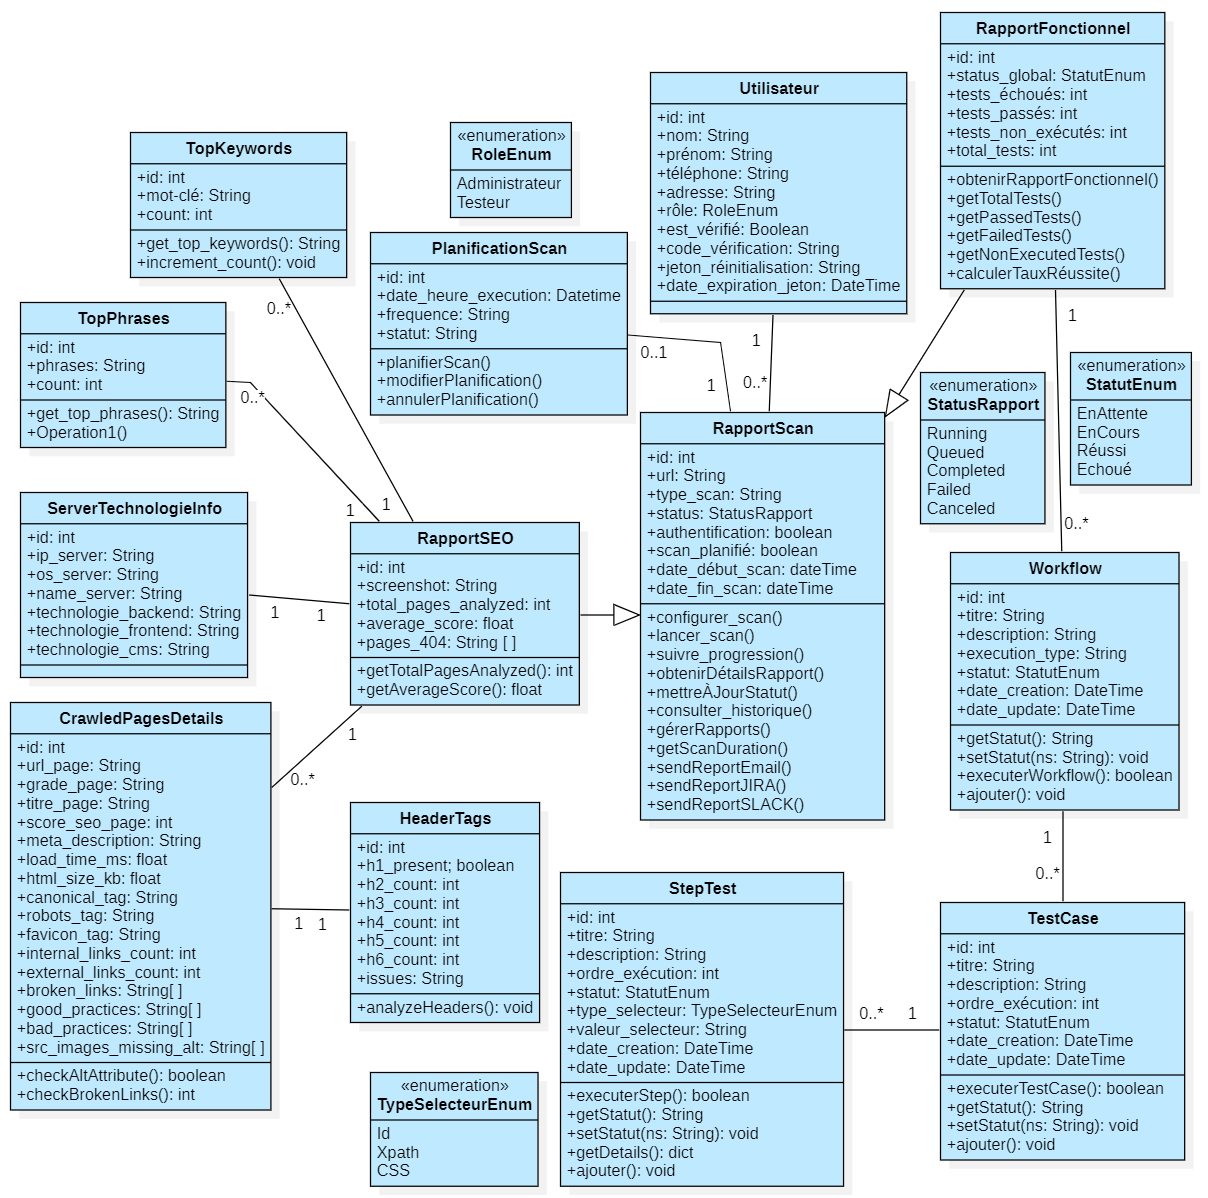
\includegraphics[width=\linewidth]{chapitres/ch4Sp2/section/sprint2.1/img/classeL2-SP2.1.png}
        \caption{Diagramme de classe du sprint 2.1}
        \label{fig:classsp2}
    \end{figure}
    \vspace{-0.7cm}
    Les principales classes modélisées du sprint 2.1 sont les suivantes:
    \begin{itemize}[label=$*$]
        \item \textbf{Utilisateur:} Classe représentant les utilisateurs du système.  
        \item \textbf{PlanficationScan:} Gère la planification des scans avec des fonctionnalités de programmation, modification et annulation des analyses automatisées.
        
        \item \textbf{RapportScan:} Classe principale pour les rapports de scan incluant la configuration, le lancement, le suivi de progression et la gestion des résultats d'analyse.
        
        \item \textbf{RapportSEO:} Spécialise les rapports pour l'analyse SEO avec des métriques spécifiques comme le nombre total de pages analysées et le score moyen.
        
        \item \textbf{RapportFonctionnel:} Représente les résultats des tests fonctionnels réalisés avec des informations sur le statut global, les différents tests effectués, et leur réussite ou échec.
        
        \item \textbf{TopKeywords:} Contient les mots-clés les plus importants extraits lors des analyses SEO, utilisés pour le suivi des performances et des tendances.
        
        \item \textbf{TopPhrases:} Contient les phrases clés les plus pertinentes issues de l'analyse SEO, servant à enrichir les rapports et améliorer le référencement.
        
        \item \textbf{ServerTechnologieInfo:} Fournit des détails sur les technologies serveur détectées, telles que les systèmes d'exploitation, CMS, frameworks front-end et back-end utilisés.
        
        \item \textbf{CrawledPagesDetails:} Représente les informations détaillées des pages web crawlées durant les scans(URL, score SEO associé, métriques de performance...).
        
        \item \textbf{HeaderTags:} Regroupe les métadonnées extraites des pages web, comme les balises Hn, les descriptions meta, et d'autres éléments influençant le référencement naturel.

        \item \textbf{Workflow:} Modélise la chaîne ou séquence d'exécution des tests automatisés, incluant la gestion du statut et des étapes du processus.
        
        \item \textbf{TestCase:} Définit un cas de test fonctionnel détaillé, incluant la description, l'ordre d'exécution, et les critères de réussite ou d'échec.
        
        \item \textbf{StepTest:} Représente une étape précise dans un scénario de test fonctionnel, avec un suivi du statut et des résultats partiels.
                
        \item \textbf{StatutEnum (énumération):} Définit les différents états possibles d'un test ou rapport (EnAttente, EnCours, Réussi, Échoué).
        
        \item \textbf{StatusRapport (énumération):} Spécifie les états des rapports de scan (Running, Queued, Completed, Failed, Canceled).
        
        \item \textbf{RoleEnum (énumération):} Définit les rôles des utilisateurs (Administrateur, Testeur).
        
        \item \textbf{TypeSelecteurEnum (énumération):} Définit les types de sélecteurs utilisés dans les tests (Id, Xpath, CSS).
    \end{itemize}
    Les associations entre classes dans Sprint 2.1 incluent:
    \begin{itemize}[label=$-$]
        \item Un \texttt{Utilisateur} peut avoir plusieurs \texttt{PlanficationScan} et \texttt{RapportScan} associés.
        \item Un \texttt{RapportFonctionnel} centralise plusieurs \texttt{Workflow}, chacun structurant l'exécution de plusieurs \texttt{TestCase}, eux-mêmes composés de plusieurs \texttt{StepTest}.
        \item Les \texttt{TopKeywords}, \texttt{TopPhrases}, \texttt{ServerTechnologieInfo} et \texttt{CrawledPagesDetails} sont liés à un \texttt{RapportSEO}.
        \item Les \texttt{HeaderTags} sont extraits pour chaque \texttt{CrawledPagesDetails}.
    \end{itemize}
    Cette modélisation structure le traitement et le suivi des tests fonctionnels et SEO, permettant une meilleure organisation et automatisation des analyses au sein du projet.



\subsubsection{Diagramme de séquence de conception du cas « Créer un scénario de test »}
Le diagramme présenté à la figure \ref{fig:add-workflow} illustre le déroulement du processus de création d’un nouveau scénario de test fonctionnel (\texttt{Workflow}). Ce processus est généralement initié par un utilisateur via l’interface de l’application et comprend la saisie des détails du scénario (nom, description). Une fois les informations saisies, le \texttt{Workflow} est créé et enregistré dans la base de données pour être exécuté ou modifié ultérieurement.

Une fois un \texttt{Workflow} créé, l'utilisateur est automatiquement redirigé vers une interface dédiée à la configuration du scénario. Cette page permet l’ajout des différents éléments constitutifs tels que les \texttt{TestCase} et les \texttt{StepTest}, tout en offrant des boutons de lancement pour exécuter directement le workflow ou ses tests associés. Cette interface assure ainsi une gestion fluide, interactive et complète du cycle de vie des scénarios de test.

\begin{figure}[H]
    \centering
    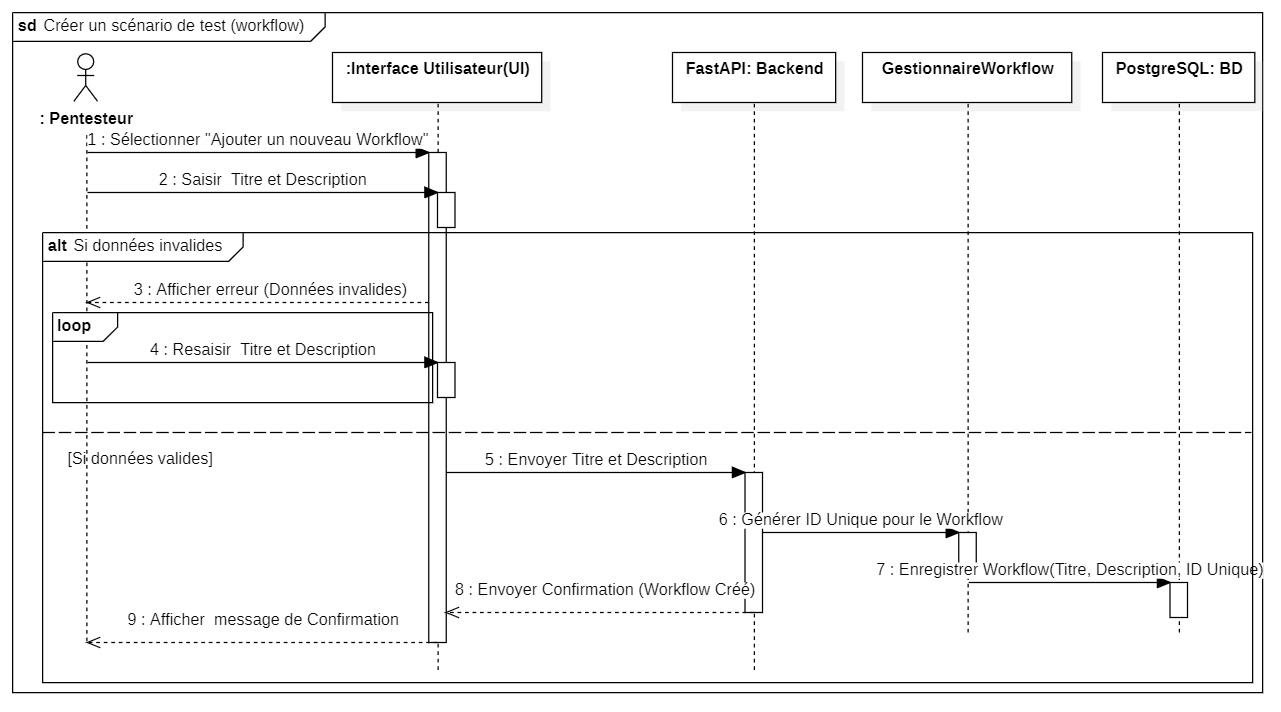
\includegraphics[width=\linewidth]{chapitres/ch4Sp2/section/sprint2.1/img/seq-workflow-creer.png}
    \caption{Diagramme de séquence de conception du cas « Créer un scénario de test »}
    \label{fig:add-workflow}
\end{figure}
\vspace{-0.4cm}

    